\documentclass[11pt]{article}

\usepackage{graphicx}

\marginparwidth 0.5in 
\oddsidemargin 0.25in 
\evensidemargin 0.25in 
\marginparsep 0.25in
\topmargin 0.0in 
\textwidth 6in \textheight 8.5in

\title{sQuire: A Web Based Collaborative Editor\\Homework 4 Individual Work\\Group 3}
\author{Rick Boss (boss2849)}

\begin{document}
\maketitle

\newpage
\tableofcontents
\newpage

\section{Compiler Functional Requirements}
        \begin{itemize}
            \item Compile project sub-modules or entire project.
            \item Compile and run code within IDE.
            \item Compile code and package to a JAR.
            \item Impose temporary code freeze during compilation.
        \end{itemize}
        
\secton{Class Diagram}
    \subsection(compiler)
    \begin{minipage}{1\textwidth}
        \begin{center}
            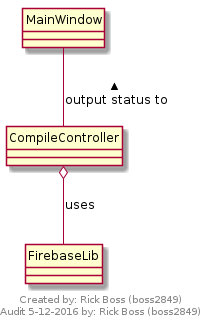
\includegraphics[width=0.7\textwidth]{uml-diagram/class-compiler}
        \end{center}
        \captionof{figure}{Use case driagram for compiler.}
    \end{minipage}

\section{Use Case Diagram}
    \subsection(Compiler)
    \begin{minipage}{1\textwidth}
        \begin{center}
            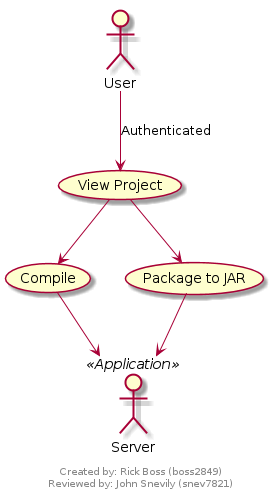
\includegraphics[width=0.7\textwidth]{uml-diagram/usecase-compiler}
        \end{center}
        \captionof{figure}{Use case driagram for compiler.}
    \end{minipage}

\section{Communication Sequence Diagram (boss2849)}
    \begin{minipage}{1\textwidth}
        \begin{center}
            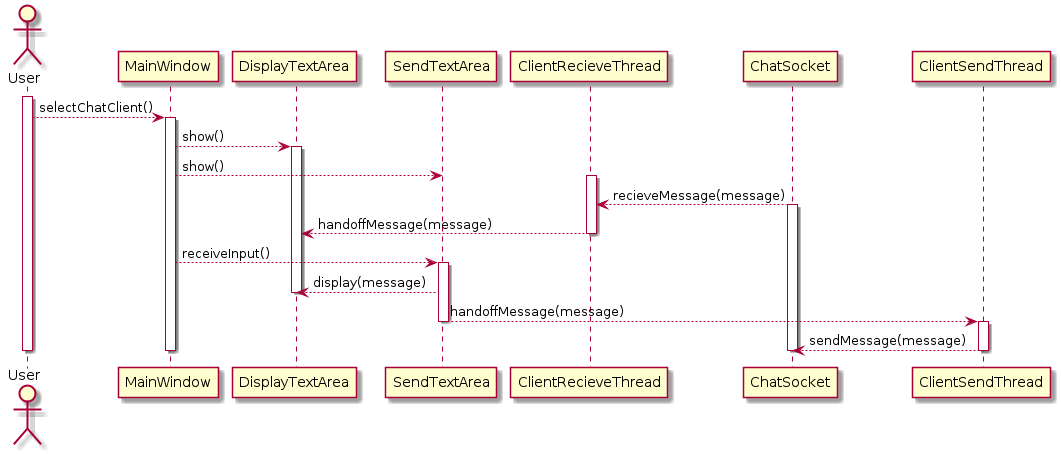
\includegraphics[width=0.7\textwidth]{diagrams/sequence-chat-client}
        \end{center}
        \captionof{figure}{Sequence diagram for chat client interaction.}
        \begin{center}
            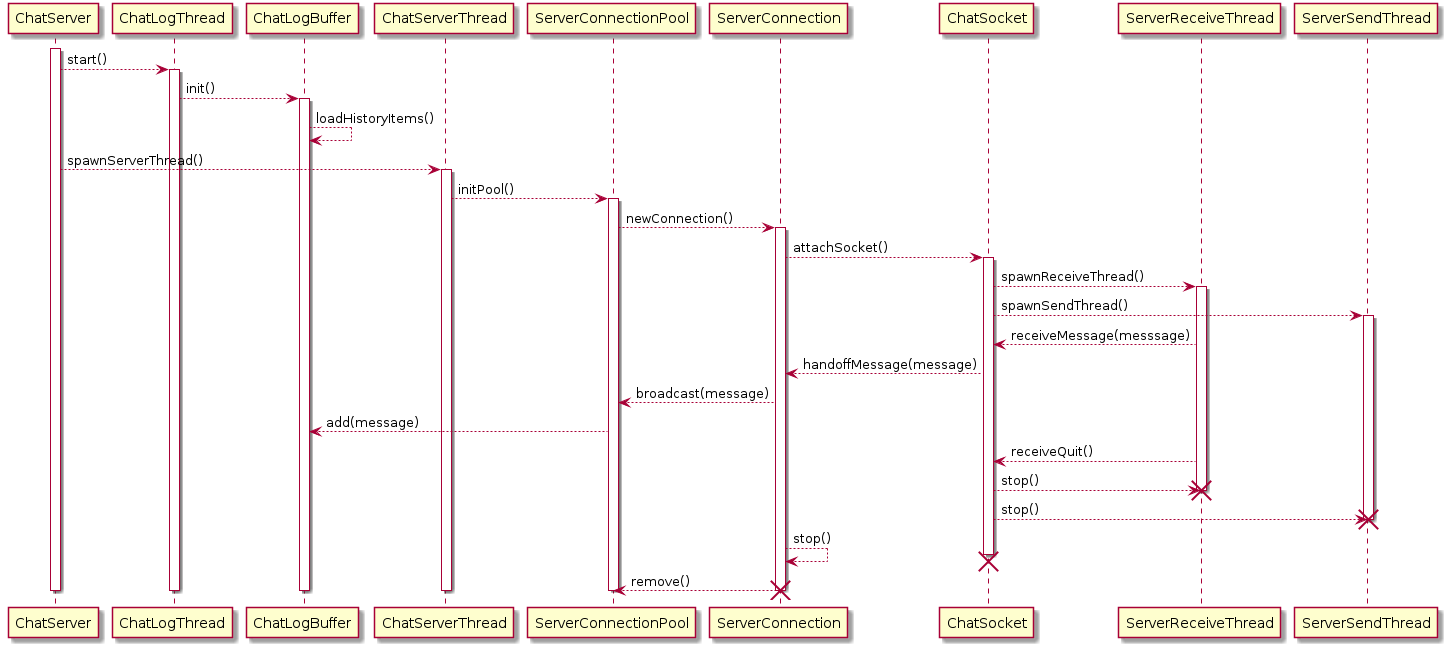
\includegraphics[width=0.7\textwidth]{diagrams/sequence-chat-server}
        \end{center}
        \captionof{figure}{Sequence diagram for chat server interaction.}
    \end{minipage}

\section{Use Case Descriptions}
\subsection{Compiler (boss2849)}
\subsubsection{Compile (boss2849)}
\begin{tabular}{ p{2cm} p{12cm} }
 \hline
 \\
 \textit{Actors:} & User \\ 
 \\
 \textit{Goals:} & Compile source \\
 \\
 \textit{Pre-conditions:} & User is logged in and viewing project. \\
 \\
 \textit{Summary:} & User requests that the code be compiled, the server compiles the code. \\
 \\
 \textit{Related use cases:} & Run, Compile To Jar \\ 
 \\
 \textit{Steps:} & \begin{enumerate}
   \item User selects ``Compile'' from ``Build'' dropdown menu for the current module.
   \item The Server receives the request to compile.
   \item The Server caches the current state of the project using the SnapshotManager and compiles it using the active CompilerPlugin.
   \item The Server returns the results of compilation to the User.
 \end{enumerate} \\
 \\
 \textit{Alternatives:} & In step 1, user chooses to compile entire project, including all sub modules. \\
 \\
 \textit{Post-conditions:} & None. \\
 \\
\hline
\end{tabular}

\subsubsection{Run (boss2849)}
\begin{tabular}{ p{2cm} p{12cm} }
 \hline
 \\
 \textit{Actors:} & User. \\ 
 \\
 \textit{Goals:} & Run the program. \\
 \\
 \textit{Pre-conditions:} & User is logged in and viewing a project. \\
 \\
 \textit{Summary:} & User chooses to run the program and the server compiles it or executes the last compilation result if no changes. \\
 \\
 \textit{Related use cases:} & Compile \\ 
 \\
 \textit{Steps:} & \begin{enumerate}
  \item User selects ``Run'' from the ``Build'' menu drop down.
  \item The Server receives the request to execute.
  \item The Server retrieves the most recent compilation from the SnapshotManager.
  \item The Server spawns a new window for the client that is the interface to the program.
 \end{enumerate} \\
 \\
 \textit{Alternatives:} & In step 3 the SnapshotManager has either an out of date compilation or no last compilation, the Server invokes the compiler to compile the project. \\
 \\
 \textit{Post-conditions:} & None. \\
 \\
\hline
\end{tabular}

\subsubsection{Package to Jar (boss2849)}
\begin{tabular}{ p{2cm} p{12cm} }
 \hline
 \\
 \textit{Actors:} & User \\ 
 \\
 \textit{Goals:} & Compile and package source to a jar\\
 \\
 \textit{Pre-conditions:} & User is signed in and viewing a project. \\
 \\
 \textit{Summary:} & User selects to build the project to a jar, the server outputs a jar on the project path. \\
 \\
 \textit{Related use cases:} & Compile \\ 
 \\
 \textit{Steps:} & \begin{enumerate}
  \item The user seclects ``Compile To Jar'' from ``Build'' dropdown menu.
  \item The Server receives the request to build a jar.
  \item The Server fetches the most recent compilation from the SnapshotManager.
  \item The Server packages the result of the last compilation to a jar and outputs it on the project path.
  \item The Server notifies the user of success.
 \end{enumerate} \\
 \\
 \textit{Alternatives:} & In step 3 the SnapshotManager has either an out of date compilation or no last compilation, the Server invokes the compiler to compile the project. In step 4 or 5, the compilation process fails and the Server notifies the user with the reason of failure. \\
 \\
 \textit{Post-conditions:} & None. \\
 \\
\hline
\end{tabular}

\subsubsection{Enable code freeze (boss2849)}
\begin{tabular}{ p{2cm} p{12cm} }
 \hline
 \\
 \textit{Actors:} & User \\ 
 \\
 \textit{Goals:} & Impose a code freeze on the project. \\
 \\
 \textit{Pre-conditions:} & User is signed in, viewing a project, and has admin rights.\\
 \\
 \textit{Summary:} & User places a code freeze on the project, preventing editing until undone. \\
 \\
 \textit{Related use cases:} & None. \\ 
 \\
 \textit{Steps:} & \begin{enumerate}
  \item The User selects ``Code Freeze'' from the dropdown menu.
  \item The Server receives the request for code freeze.
  \item The Server restricts all editing of project files.
 \end{enumerate} \\
 \\
 \textit{Alternatives:} & None. \\
 \\
 \textit{Post-conditions:} & None. \\
 \\
\hline
\end{tabular}

\end{document}
